\documentclass[handout, t, aspectratio=169]{beamer}
 
\usepackage[utf8]{inputenc}
\usepackage{times}
\usepackage[T1]{fontenc}
\usepackage[spanish]{babel}
\usetheme{Madrid}
\hypersetup{
    colorlinks=true,
    linkcolor=blue,
    filecolor=magenta,      
    urlcolor=cyan,
}
 
 \newtheorem{definicion}[theorem]{Definición}
 
%Information to be included in the title page:
\title{Bases de Datos Temporales}
\author{F. Badaloni, D. Giordana}
\institute{FCEIA, UNR}
\date{8/5/2019}

\begin{document}

\frame{\titlepage}
\section{Introducción}
\begin{frame}{¿Qué queremos hacer?}
    \begin{itemize}
    \item El tiempo es un aspecto importante para describir el mundo real. \pause
    \begin{itemize}
        \item Los objetos y las relaciones entre ellos existen a través del tiempo.
    \end{itemize}\pause
    \item La habilidad de \textbf{modelar} la dimensión temporal del mundo real es fundamental para resolver muchos problemas:
    \begin{itemize}
        \item Econometría.\pause
        \item Bancos.\pause
        \item Control de inventario.\pause
        \item Contabilidad.\pause
        \item Leyes.\pause
        \item Registros médicos.\pause
        \item Sistemas de reservas de vuelos.\pause
        \item ...
    \end{itemize}\pause
    \item Las bases de datos convencionales representan el estado de una \textit{empresa} en un momento específico:\pause
    \begin{itemize}
        \item El presente.\pause
    \end{itemize}
    \item A medida que la base de datos se modifica, las versiones anteriores se pierden.
\end{itemize}
\end{frame}

\begin{frame}{Antes de continuar}
    \begin{itemize}
        \item Antes de continuar hay que establecer algunos conceptos.\pause
        \begin{definicion}{User-Defined time}
        El \textit{tiempo definido por el usuario} es un atributo no interpretado de fecha o tiempo.
        \end{definicion}\pause
        \item Es decir, no tiene una semántica "temporal" para la base de datos.\pause
        \item Está a la par de tipos como "dinero" y entero.\pause
        \item Estos tipos no tienen \textit{query}s especiales.\pause
        \item Puede ser usado para representar \textbf{cumpleaños} o \textbf{fechas de nacimiento}.\pause
        \item El estándar SQL soporta estos tipos hace más de 25 años.\pause
        \begin{itemize}
            \item \textit{datetime}, \textit{interval}.
        \end{itemize}
    \end{itemize}
\end{frame}

\begin{frame}{¿Qué es una base de datos temporal?}
    \begin{itemize}
        \item Generalmente se usa el modificador \textbf{temporal} para indicar que un concepto involucra algún aspecto del tiempo.\pause
        \item Cuando se hable de bases de datos temporales \alert{NO} se incluye el uso de tiempos definidos por le usuario.\pause
        \item Pero no existe consenso al definir base de datos temporales.\pause
        \begin{itemize}
            \item Hay distintos niveles de especificidad.
        \end{itemize}\pause
        \item Algunos investigadores consideran que para que una base de datos pueda llamarse temporal debe soportar \textbf{tiempo de transacción} y \textbf{tiempo de validez}.\pause
        \item Por otra parte otros académicos sustentan que con soportar alguna de estas características es suficiente.\pause
        
        \item A este tipo de bases de datos también se las conoce como:
        \begin{itemize}
            \item Orientadas al tiempo. (Time-Oriented)
        \end{itemize}
    \end{itemize}
\end{frame}

\begin{frame}{La estructura del tiempo 1}
    \begin{itemize}
        \item Inicialmente se asume que el tiempo corre en una dimensión.\pause
        \item Los trabajos en la \textit{lógica temporal} se centraron en dos modelos estructurales del tiempo:\pause
        \begin{itemize}
            \item Modelo Lineal.\pause
            \item Modelo de ramificación.\pause
        \end{itemize}
        
        \item En el \textbf{modelo lineal} el tiempo avanza del pasado al futuro de forma ordenada.\pause
        \begin{figure}
            \centering
           \includegraphics[scale=0.5]{Temporales/assets/linear_time.png}
        \end{figure}
    \end{itemize}
\end{frame}

\begin{frame}{La estructura del tiempo 2}
    \begin{itemize}
        \item El modelo de ramificación también es conocido como el \textbf{modelo de los futuros posibles}.\pause
        \item En este modelo el tiempo:\pause
        \begin{itemize}
            \item es lineal del pasado hasta el presente.\pause
            \item se divide en varias lineas de tiempo (futuros posibles).\pause
        \end{itemize}
        \item A su vez en una ramificación pueden haber varias ramificaciones.\pause
        \item La estructura de la ramificación tiene como raíz el presente.\pause
        \begin{figure}
            \centering
           \includegraphics[scale=0.35]{Temporales/assets/branched_time.png}
        \end{figure}
    \end{itemize}
\end{frame}

\begin{frame}{La estructura del tiempo 3}
    \begin{itemize}
        \item El modelo más general de tiempo en la lógica temporal representa el tiempo como un \textbf{conjunto arbitrario con un orden parcial}.\pause
        \item Se pueden agregar axiomas al modelo para refinarlo más:\pause
        \begin{itemize}
            \item El tiempo lineal puede ser especificado con un orden total.
        \end{itemize}\pause
        \item Los modelos temporales son más complejos que los modelos espaciales.\pause
        \begin{itemize}
            \item Para representar el espacio un modelo lineal alcanza.
        \end{itemize}\pause
        \item A partir de ahora supondremos el uso del modelo lineal.
    \end{itemize}
\end{frame}

\begin{frame}{La densidad del tiempo}
    \begin{itemize}
        \item Se pueden agregar axiomas a la lógica temporal para caracterizar la \textbf{densidad} de una linea del tiempo.\pause
        \item Dentro de esta clasificación podemos tener dos tipos principales de modelos:\pause
        \begin{itemize}
            \item Modelos discretos.\pause
            \item Modelos continuos.
        \end{itemize}
    \end{itemize}
\end{frame}

\begin{frame}{Modelos Discretos}
    \begin{itemize}
        \item Los \textbf{modelos discretos} son isomorfos a los números naturales.\pause
        \begin{itemize}
            \item Cada punto en el tiempo tiene un único sucesor.
        \end{itemize}\pause
        \item Cada número natural se corresponde con una unidad de tiempo no descomponible de duración arbitraria.\pause
        \item Estas unidades de tiempo no descomponibles se denominan \textbf{\textit{chronon}}\pause
        \item Un chronon es la menor duración de tiempo que puede ser representada en este modelo.\pause
        \begin{itemize}
            \item No son puntos sino segmentos en una linea del tiempo.
        \end{itemize}
    \end{itemize}    
\end{frame}

\begin{frame}{Modelos Continuos}
    \begin{itemize}
        \item Los \textbf{modelos densos} del tiempo son isomorfos a los \textit{racionales} o a los \textit{reales}. \pause
        \begin{itemize}
            \item Entre cualquiera dos momentos del tiempo existe otro momento.
        \end{itemize}\pause
        \item Los \textbf{modelos continuos} son isomorfos a los \textit{reales} \pause
        \begin{itemize}
            \item No contienen huecos entre dos momentos.
        \end{itemize}\pause
        \item Cada número real se corresponde con un "punto" del tiempo.
    \end{itemize}    
\end{frame}

\begin{frame}{¿Qué modelo elegir?}
    \begin{itemize}
        \item El tiempo en si mismo es generalmente percibido como continuo.\pause
        \item No obstante, la mayoría de las propuestas para agregar una dimensión temporal a una base de datos están basadas en modelos discretos del tiempo.\pause
        \item ¿Por qué?:\pause
    \end{itemize}
    \begin{enumerate}
        \item La medición del tiempo es inherentemente imprecisa\pause
        \begin{itemize}
            \item Los instrumentos de cronometraje invariablemente reportan la ocurrencia de eventos en términos de crhonons, no "puntos" de tiempo.\pause
            \item Los eventos llamados "\textit{instantaneos}" pueden en el mejor de los casos medirse como si hubieran ocurrido en un chronon.\pause
        \end{itemize}
        \item Las formas más naturales de la lengua son compatibles con el modelo discreto.\pause
        \begin{itemize}
            \item Las \textbf{11:00 A.M.} abarca un minuto de duración.
        \end{itemize}\pause
        \item Los conceptos de chronon e intervalos permiten modelar eventos que no son instantáneos, pero tienen duración.\pause
        \item Cualquier implementación de un modelo de datos con una dimensión temporal en algún punto será discretizado al codificar el tiempo.
    \end{enumerate}
\end{frame}

\begin{frame}{...}
    \begin{itemize}
        \item Y ahora viajemos un poco al futuro.\pause
        \begin{figure}
            \centering
            \includegraphics[scale=0.2]{Temporales/assets/travel-the-future.jpg}
        \end{figure}\pause
        \item Existen muchos conceptos que no podemos abarcar en este momento.\pause
        \begin{itemize}
            \item Distancia entre momentos.\pause
            \item Tiempos absolutos y tiempos relativos.\pause
            \item Representaciones del tiempo.\pause
            \item Indeterminación.\pause
            \item ...
        \end{itemize}
    \end{itemize}
\end{frame}

\begin{frame}{¿Cómo llevamos esto a las bases de datos?}
    \begin{itemize}
        \item Para explicar los conceptos se usará como ejemplo el modelo relacional en tablas.\pause
        \begin{figure}
            \centering
             \includegraphics[scale=0.5]{Temporales/assets/db_table.jpg}
        \end{figure}
    \end{itemize}
\end{frame}

\begin{frame}{Base de datos Snapshot}
    \begin{itemize}
        \item Llamamos base de datos Spapshot a cualquier base de datos que no soporta capacidades temporales.\pause
        \begin{itemize}
            \item Aunque puede tener Tiempos definidos por el usuario.
        \end{itemize}\pause
        \item Es fácil ver estas bases de datos como máquinas de estado finitas.\pause
        \begin{figure}
            \centering
            \includegraphics[scale=0.3]{Temporales/assets/state_machine.jpg}
        \end{figure}\pause
        \item Los cambios "destruyen" los datos anteriores.
    \end{itemize}
\end{frame}

\begin{frame}{Tiempo Válido}
    \begin{itemize}
        \item El \textbf{\textit{tiempo válido}} de un hecho es el tiempo cuando el hecho es verdadero en la realidad modelada.\pause
        \item Un hecho puede tener asociado cualquier número de instantes e intervalos de tiempo.\pause
        \item Los tiempos validos suelen ser ingresados por el usuario.\pause
        \item A este término también se lo suele conocer como:
        \begin{itemize}
            \item Real-World time.\pause
            \item Logical time.\pause
            \item Data time.
        \end{itemize}
    \end{itemize}
\end{frame}

\begin{frame}{Tiempo de transacción}
    \begin{itemize}
        \item Un hecho de la base de datos es almacenado en la base de datos en algún punto del tiempo.\pause
        \item Este hecho es "actual" hasta que que es lógicamente eliminado.\pause
        \item El \textit{\textbf{tiempo de transacción}} de un hecho de una base de datos es el tiempo cuando un hecho es actual y puede ser "recuperado".\pause
        \item Como consecuencia:\pause
        \begin{itemize}
            \item Tienen una duración.\pause
            \item No se pueden extender en el futuro.\pause
            \item Es imposible cambiar el pasado.
        \end{itemize}
    \end{itemize}
\end{frame}

\begin{frame}{Agregando tiempo a las bases de datos}
    \begin{itemize}
        \item Una base de datos temporal soporta tiempo válido o tiempo de transacción.
    \end{itemize}\pause
    \begin{figure}
        \centering
        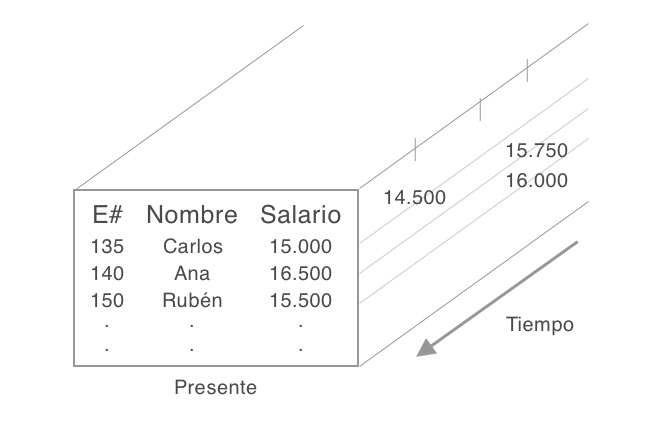
\includegraphics[scale=0.4]{Temporales/assets/temporal_dimension.jpg}
    \end{figure}
\end{frame}

\begin{frame}{Tipos de bases de datos temporales}
    \begin{itemize}
        \item Base de datos de tiempo válido\pause
        \begin{itemize}
            \item Soporta tiempo válido.
            \item también son conocidas como bases de datos históricas.
        \end{itemize}
        \pause
        \item Base de datos de tiempo de transacción\pause
        \begin{itemize}
            \item Soporta tiempo de transacción.\pause
            \item También son conocidas como:\pause
            \begin{itemize}
                \item Rollback databases.\pause
                \item Immutable databases.\pause
            \end{itemize}
        \end{itemize}
        
        \item Bases de datos \textit{temporales}\pause
        \begin{itemize}
            \item Soportan ambos tipos de tiempos.\pause
            \item Permiten los viajes en el tiempo.
        \end{itemize}\pause
        \item Dependiendo la cantidad de tiempos que soportan son uni-temporales o bi-temporales.
    \end{itemize}
\end{frame}

\begin{frame}{Querys Temporales}
    \begin{itemize}
        \item Existen tres tipos de querys:
    \end{itemize}\pause
    \begin{enumerate}
        \item \textbf{Snapshot querys}:\pause
        \begin{itemize}
            \item Solicita datos a la base de datos en el presente.\pause
        \end{itemize}
        \item \textbf{Temporal querys}:\pause
        \begin{itemize}
            \item Solicita datos a la base de datos en cualquier momento.
        \end{itemize}\pause
        \item \textbf{Time Travel querys}:\pause
        \begin{itemize}
            \item Retorna a una version anterior de la base de datos para ver la base de datos.
        \end{itemize}
    \end{enumerate}
\end{frame}

\section{SQL 2011}

\begin{frame}{SQL 2011}
\begin{itemize}
    \item La versión 2011 de SQL, publicada en diciembre de 2011 extiende el estándar con funcionalidades temporales.\pause
    \item Esta extensión se basa en el agregado de períodos temporales a las tablas.\pause
    \item Dos tipos de períodos: de aplicación de usuario (para tiempos de validez) y de versionado de sistema (para tiempos de transacción).\pause
    \item Agrega predicados temporales sobre períodos.\pause
    \item Este \href{https://cs.ulb.ac.be/public/_media/teaching/infoh415/tempfeaturessql2011.pdf}{paper} resume las funcionalidades temporales de SQL 2011.
\end{itemize}
\end{frame}

\begin{frame}{SQL 2011: Períodos}
    \begin{itemize}
        \item Los períodos se definen con dos columnas temporales (Date o Timestamp) de la tabla. \pause
        \item Se prefirió esta forma en lugar de un tipo nuevo ya que es la que permite migrar más fácilmente sistemas previos al estándar.\pause
        \item \textbf{Períodos cerrado-abierto}: un período representado por dos datos de tipo temporal incluye al momento de inicio pero no al de finalización. \pause
        \begin{itemize}
            \item Va a facilitar propiedades algebraicas. 
        \end{itemize}
    \end{itemize}
\end{frame}

\begin{frame}[fragile]{SQL 2011: Aplicación de Usuario}
    \begin{verbatim}
    CREATE TABLE Estudiante (
    Legajo INTEGEER,
    EStart DATE,
    EEnd DATE,
    ECarrera INTEGER,
    PERIOD FOR EPeriod (EStart, EEnd)
    )
    \end{verbatim}\pause
    \begin{itemize}
        \item Modificables por el usuario.\pause
        \item \textit{INSERT} es básicamente igual.\pause
    \end{itemize}
    \begin{verbatim}
    INSERT INTO Estudiante
    VALUES (1234, DATE '2013-03-01', DATE '2018-12-20', 1)
    \end{verbatim}
\end{frame}

\begin{frame}[fragile]{SQL 2011: Aplicación de Usuario}
    \begin{verbatim}
    UPDATE Estudiante
        FOR PORTION OF EPeriod
            FROM DATE  DATE '2015-04-01'
            TO DATE '2015-05-01'
    SET Carrera = 2
    WHERE Legajo = 1234
    \end{verbatim}
    \pause
    \begin{itemize}
        \item Un \textit{UPDATE} puede tomar un período y resultar en más de una fila (hasta 3), dependiendo del periodo anterior y el nuevo.\pause
        \item Similarmente, un \textit{DELETE} puede borrar un dato en un subperíodo de su validez.\pause
        \item Para triggers: la fila con carrera = 2 es la actualizada, las otras dos son insertadas.
    \end{itemize}
\end{frame}

\begin{frame}{SQL 2011: Claves Primarias}
    \begin{itemize}
        \item En el ejemplo anterior, si la PK era el legajo, quedamos con duplicación. Tenemos que incluir el período en la PK.\pause
        \item Para evitar superposiciones (la forma temporal de los duplicados) agregamos a la definición \textit{WITHOUT OVERLAPS}.\pause
        \item También hay otras nuevas restricciones de integridad temporal: podes pedir que un estudiante no pueda estudiar una carrera que no existía en ese período.
    \end{itemize}
\end{frame}

\begin{frame}[fragile]{SQL 2011: Predicados}
    \begin{itemize}
        \item X OVERLAPS Y: dos períodos tienen al menos un punto temporal en común. Es simétrico\pause
        \item X CONTAINS Y: Todo punto de Y está en X.\pause
        \item X PRECEDES Y, X SUCCEEDS Y\pause
        \item X INMEDIATLY PRECEDES Y, X INMEDIATLY SUCCEEDS Y\pause
        \item X EQUALS Y \pause
    \end{itemize}
    \begin{verbatim}
    SELECT Legajo, Carrera, sys_start, sys\_end
    FROM Estudiante WHERE Legajo = 1
        AND EPeriod CONTAINS DATE '2018-05-08'
    \end{verbatim}
\end{frame}

\begin{frame}{SQL 2011: Versionado de Sistema}
    \begin{itemize}
        \item El otro tipo de períodos es de versionado de sistema. Las tablas declaradas con versionado de sistema, tienen campos temporales de nombre fijo (sys\_start y sys\_end) que el usuario no puede modificar. Son definidas por el sistema al momento de realizar otras operaciones. Se declaran con WITH SYSTEM VERSIONING.\pause
        \item Cualquier UPDATE o DELETE automáticamente preservan el estado anterior de la fila. \pause
        \item Dos tipos de filas: de sistema actual e históricas.\pause
        \item Solo puedo efectuar UPDATE y DELETE el sistema actual, no sobre versiones históricas.\pause
        \item Las restricciones de integridad son mas sencillas. Cualquier restriccion que es chequeada y se cumple en el sistema actual, heredará la propiedad cuando pase a ser una versión histórica.\pause
        \item Podemos usar al mismo tiempo períodos de aplicación de usuario y versionado de sistema: bitemporales.
    \end{itemize}
\end{frame}

\begin{frame}[fragile]{SQL 2011: Viajar al pasado}
    \begin{verbatim}
    SELECT Legajo, Carrera, sys_start, sys\_end
    FROM Estudiante FOR SYSTEM TIME
        AS OF TIMESTAMP '2017-05-01 00:00:00'
    \end{verbatim}\pause
    \begin{verbatim}
    SELECT Legajo, Carrera, sys_start, sys_end
    FROM Estudiante FOR SYSTEM TIME
        FROM TIMESTAMP '2017-05-01 00:00:00'
        TO TIMESTAMP '2017-06-01 00:00:00'
    \end{verbatim}\pause
    \begin{verbatim}
    SELECT Legajo, Carrera, sys_start, sys_end
    FROM Estudiante FOR SYSTEM TIME
        BETWEEN TIMESTAMP '2017-05-01 00:00:00'
        AND TIMESTAMP '2017-06-01 00:00:00'
    \end{verbatim}
\end{frame}

\begin{frame}[fragile]{SQL 2011: Viajar al pasado}
    \begin{itemize}
        \item Podemos consultar versiones históricas con esta sintaxis nueva.\pause
        \item Una query sin especificar tiempo es equivalente a FOR SYSTEM TIME AS OF CURRENT TIMESTAMP.\pause
        \item FROM ... TO ... es Cerrado-Abierto mientras que BETWEEN ... AND ... es Cerrado-Cerrado.
    \end{itemize}
\end{frame}

\begin{frame}[fragile]{SQL 2011: Todas las versiones}
    \begin{verbatim}
    SELECT Legajo, Carrera, sys\_start, sys\_end
    FROM Estudiante FOR SYSTEM TIME BETWEEN
        TIMESTAMP '0001-01-01 00:00:00' AND
        TIMESTAMP '9999-12-31 23:59:59'
    \end{verbatim}
\end{frame}

\section{Estado del arte}

\begin{frame}{Estado del Arte: Bases de Datos Temporales Imperfectas}
    \begin{itemize}
        \item Las referencias temporales en el lenguaje natural son vagas. La representación y tratado de las incertezas provenientes de esto son una rama de estudio activa de las Bases de Datos Temporales.\pause
        \item \href{https://ddcm.ugent.be/}{Grupo DDCM} (Database, Document and Content Management) de la Universidad de Gante, Bélgica.\pause
        \item \href{https://link.springer.com/chapter/10.1007/978-3-319-00954-4_9}{Paper}: Aspects of Dealing with Imperfect Data in Temporal Databases
    \end{itemize}
\end{frame}

\begin{frame}{Estado del Arte: Compresión de Datos Redundantes}
    \begin{itemize}
        \item Guardar todas las snapshots completas obviamente es redundante. En este paper, se discute como compactar la información guardada haciendo merges. Arman un modelo teórico para poder probar que todos los estados individuales son derivables del merge. \pause
        \item \href{https://ddcm.ugent.be/}{Grupo DDCM} (Database, Document and Content Management) de la Universidad de Gante, Bélgica.\pause
        \item \href{https://link.springer.com/article/10.1007/s00778-018-0535-4}{Paper}: Compact representations of temporal databases
    \end{itemize}
\end{frame}

\begin{frame}{Estado del Arte: Timeline Index}
    \begin{itemize}
        \item Similarmente al lugar que ocupaban los realms en el Álgebra de Rose, se esta investigando diferentes beneficios que puede tener usar al recta temporal como índice universal. En este caso, se usa para definir operaciones de agregado temporales eficientes.\pause
        \item \href{https://www.inf.unibz.it/idse/}{IDSE} Center for Information and Database Systems Engineering\pause
        \item \href{https://link.springer.com/chapter/10.1007\%2F978-3-319-64367-0_7}{Paper}: Sweeping-Based Temporal Aggregation
    \end{itemize}
\end{frame}

\begin{frame}{Y ahora ...}
    \begin{figure}
        \includegraphics[scale=0.18]{Temporales/assets/to_be_continued.jpg}
        \label{fig:to_be_continued}
    \end{figure}
\end{frame}

\end{document}